% XCircuit output "1.3.tex" for LaTeX input from 1.3.eps
\def\putbox#1#2#3#4{\makebox[0in][l]{\makebox[#1][l]{}\raisebox{\baselineskip}[0in][0in]{\raisebox{#2}[0in][0in]{\scalebox{#3}{#4}}}}}
\def\rightbox#1{\makebox[0in][r]{#1}}
\def\centbox#1{\makebox[0in]{#1}}
\def\topbox#1{\raisebox{-0.60\baselineskip}[0in][0in]{#1}}
\def\midbox#1{\raisebox{-0.20\baselineskip}[0in][0in]{#1}}
   \scalebox{1}{
   \normalsize
   \parbox{2.78125in}{
   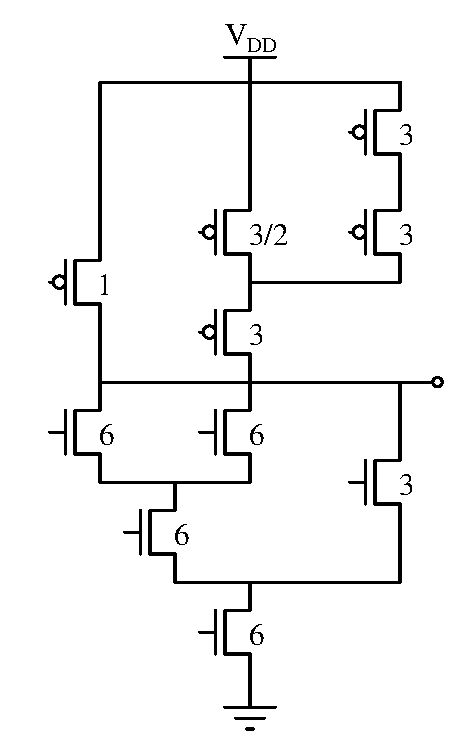
\includegraphics[scale=1]{1.3.eps}\\
   % translate x=544 y=732 scale 0.38
   \putbox{2.06in}{3.95in}{1.20}{A}%
   \putbox{2.06in}{3.29in}{1.20}{B}%
   \putbox{1.06in}{3.29in}{1.20}{C}%
   \putbox{1.06in}{2.62in}{1.20}{D}%
   \putbox{0.06in}{2.95in}{1.20}{E}%
   \putbox{0.06in}{1.95in}{1.20}{A}%
   \putbox{1.06in}{1.95in}{1.20}{B}%
   \putbox{2.06in}{1.62in}{1.20}{D}%
   \putbox{0.56in}{1.29in}{1.20}{C}%
   \putbox{1.06in}{0.62in}{1.20}{E}%
   } % close 'parbox'
   } % close 'scalebox'
   \vspace{-\baselineskip} % this is not necessary, but looks better
